\documentclass[letterpaper, 12pt] {article}

\usepackage{amsmath}
\usepackage{graphicx}
\usepackage{wrapfig}
\usepackage[margin=2cm]{geometry}
\usepackage[export]{adjustbox}
\usepackage{caption}
\usepackage{subcaption}
\usepackage[spanish, es-tabla]{babel}
\usepackage[T1]{fontenc}
\usepackage[utf8]{inputenc}
\usepackage{physics}


\usepackage{xcolor} 
	\definecolor{bone}{RGB}{253,255,224}  %hueso
	\definecolor{lgreen}{RGB}{146,197,130} %light green,
	\definecolor{lblue}{RGB}{134,165,169} %light blue
	\definecolor{lgray}{RGB}{118,118,118} %light gray
	\definecolor{dgreen}{RGB}{83,111,80}%dark green
	
\usepackage[colorlinks, linkcolor=lblue]{hyperref}
\graphicspath {{images/}}	
	
\usepackage[most]{tcolorbox}
\tcbset{%colback=blue!55!green, colframe= blue!55!green,
		colback=lgreen, colframe= dgreen,
		  colbacktitle = green!50!blue, sharp corners = downhill, 
	  fonttitle=\bfseries , boxrule = .75mm }%,leftrule = 5mm}




\begin{document}
{\LARGE \bf Sección 3.4.1 \\ 
 Extinción por una placa de partículas  }\\
{\large Urrutia Aguiano, Jonathan Alexis}\\

Supongamos una colección de partículas colocadas en la región semi infinita definida por los intervalos $0<z<h$, $-\infty<x<\infty$ y $-\infty<y<\infty$, en donde las partículas se encuentran distribuídas \emph{casi} uniformemente. Si una onda plana  polarizada dada por

\begin{equation}
{E}_i  = E_0 e^{ikz}\hat{e}_x, \label{eq:E_i}
\end{equation}


incide de forma normal a la placa de partículas (ver fig. \ref{fig:placa}), el campo eléctrico transmitido $\vec{E}_t$, en el punto $P$, es la suma del campo incidente y el campo esparcido por cada una de las partículas en el punto $\vec{R}_j$, denotado por $\vec{E}_{sj}$. Esto es
\begin{equation}
\vec{E}_t = \vec{E}_i + \sum_j \vec{E}_{sj}, \label{eq:E_t}
\end{equation}
donde se considera que
\begin{align}
\vec{E}_{sj} = \frac{e^{k R_j}}{-ikR_j}\vec{X}_j (\hat{e}_j)E_0 e^{ikz_j}, \\
\vec{R_j} = - [x_j \hat{e}_x + y_j \hat{e}_y + (z_j-d)\hat{e}_z ] = R_j \hat{e}_j.\label{eq:RenP}
\end{align}
Asimismo,  $\vec{X}_j(\hat{e}_j) = (S_2 \cos\varphi_j + S_3\sin\varphi_j) \hat{e}_{\parallel s j} + (S_4 \cos\varphi_j + S_1 \sin\varphi_j) \hat{e}_{\perp s j }$ y en coordenadas polares depende de las variables $\varphi_j$ y $\theta_j$, ya que $\hat{e}_{\parallel s j} = \hat{e}_{\theta_i}$ y $\hat{e}_{\perp s j } = \hat{e}_{\varphi j}$

\begin{figure}[h!]
\centering
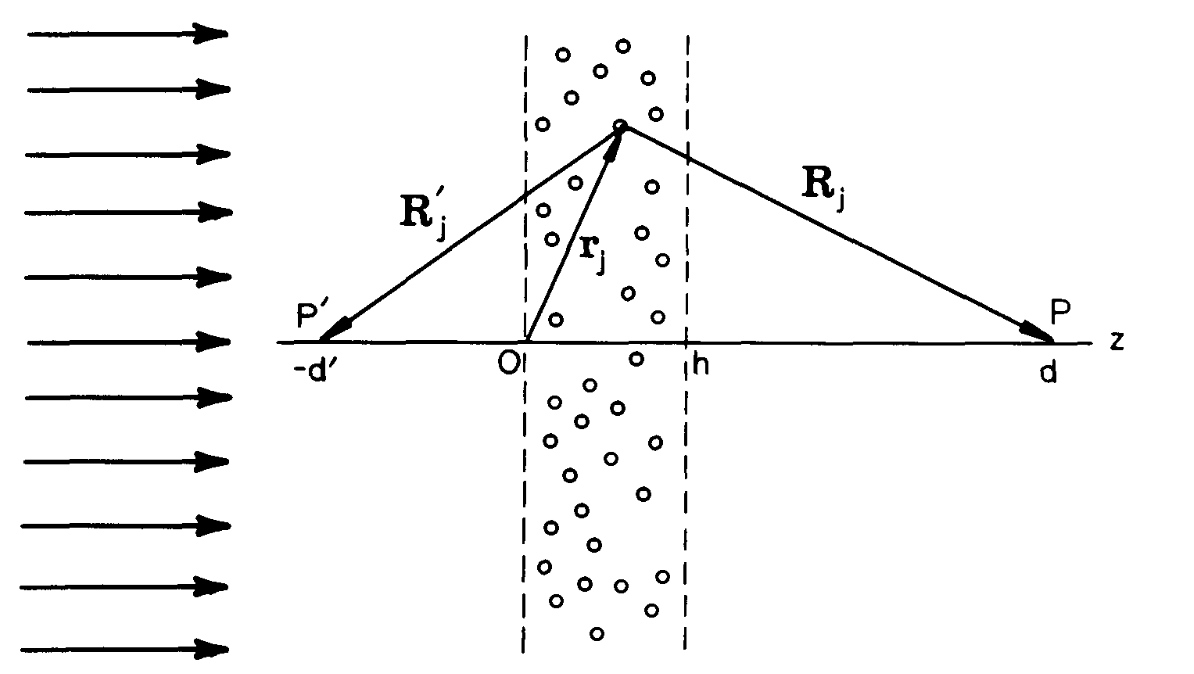
\includegraphics[width=.5\linewidth]{placa}
\caption{\scriptsize Placa semi infinita de grosor $h$. El punto $P$ se encuntra a una distancia $d$ del origen.}
\label{fig:placa}
\end{figure}

Suponiendo además que el número de partículas por volumen $n$ es tal que permite aproximar la suma de la ec. (\eqref{eq:E_t}) mediante una integral, que todas las partículas en la placa son idénticas y, dado que la onda plana incide de manera normal a la placa, $\vec{X}_j(\hat{e}_j) = \vec{X}(\hat{e})$. Entonces el campo esparcido se escribe como
\begin{align}
\sum_j \vec{E}_{sj} &\approx E_0 n
							 \int_0^h dz e^{ikz} 
							 \int_{-\infty}^\infty dy
							 \int_{-\infty}^\infty dx \frac{\vec{X}(\hat{e})}{-ikR} e^{ikR},\label{eq:E_s}  \\
				& = E_0 n \int_0^h dz e^{ikz}  \int_{-\infty}^\infty dy I_x(y,z),\\
				&= E_0 n \int_0^h dz e^{ikz}  I_y(z),
\end{align}
donde $I_x$ es el resultado de la integral en la variable $x$ y a su vez $I_y$ el resultado de la integral en la variable $y$. Sustituyendo la ec. (\ref{eq:RenP}) en (\ref{eq:E_s}) se obtiene que 
\begin{align}
\sum_j \vec{E}_{sj} &\approx E_0 n
							 \int_0^h dz e^{ikz} 
							 \int_{-\infty}^\infty dy
							 \int_{-\infty}^\infty dx 
			\frac{\vec{X}(\hat{e})    e^{ik\sqrt{x^2 + y^2 + (d-z)^2}}}
			{-ik \sqrt{x^2 + y^2 + (d-z)^2}}.
\end{align}
En secciones anteriores se suposo que $k r \gg 1$ pero como $r=d$, entonces $k\gg1$. Entonces es posible calcular $I_x$ mediante el teorema de fase estacionaria\footnote{Sean $f$ y $g$  funciones que permita su expansión en series de Taylor en el intervalo $[a,b]$, ($g$  con valores en los reales) y que en $c\in[a,b]$ se cumpla que $g'(c) = 0$,$g''(c) \not= 0$, $f(c)\not= 0$ y que $g$ sea distinto de cero en todo el intervalo. Si $\alpha \gg 1$, entonces
\begin{equation}
\int_a^b f(t) e^{\alpha g(t)} \approx f(c) e^{i\alpha g(c)}\sqrt{\frac{2\pi}{\alpha |g''(c)|}}e^{i\pi\mu/4},
\end{equation}
 con $\mu = sign(g''(c))$}, identificando 
 \begin{align*}
 \alpha &\rightarrow k, \\
 g(x) &\rightarrow \sqrt{x^2 + y^2 + (d-z)^2}, \\
 f(x) &\rightarrow  \frac{\vec{X}(\hat{e}) }{-ik \sqrt{x^2 + y^2 + (d-z)^2}},
 \end{align*}
y como $g'(x)=0$ si $x=0$ y $g''(0) = \frac{1}{\sqrt{y^2+(d-z)^2}}$, se obtiene que
\begin{align}
I_x (y,z) = \frac{(\vec{X}(\hat{e}))_{x=0} }{-ik (y^2+(d-z)^2)^{1/4}} \sqrt{\frac{2\pi}{k}} e^{i\pi/4}   e^{ik\sqrt{y^2+(d-z)^2}}.  \label{eq:Ix}
\end{align}
Como $I_y (z) = \int_{-\infty}^{\infty} I_x(y,z) dy$, se puede utilizar nuevamente el teorema de fase estacionaria, identificando 
 \begin{align*}
 \alpha &\rightarrow k, \\
 g(y) &\rightarrow \sqrt{ y^2 + (d-z)^2}, \\
 f(y) &\rightarrow  \frac{(\vec{X}(\hat{e}))_{x=0} }{-ik (y^2+(d-z)^2)^{1/4}} \sqrt{\frac{2\pi}{k}} e^{i\pi/4},
 \end{align*}
y como $g'(y)=0$ si $y=0$ y $g''(0) = \frac{1}{|d-z|}$, entonces

\begin{align}
I_y (z) &= \left( \frac{(\vec{X}(\hat{e}))_{x,y=0} }{-ik ((d-z)^2)^{1/4}} \sqrt{\frac{2\pi}{k}} e^{i\pi/4} \right) \sqrt{\frac{2\pi |z-d|}{k}}e^{i\pi/4}e^{ik|d-z|}  \notag \\
	&= - \frac{2\pi}{k^2} (\vec{X}(\hat{e}))_{x,y=0} e^{ik|d-z|}, \label{eq:Iy}
\end{align}
por lo que el campo esparcido está dado por la expresión
\begin{align}
\sum_j \vec{E}_{sj} &\approx - E_0 n  \frac{2\pi}{k^2} (\vec{X}(\hat{e}))_{x,y=0}
					\int_0^h e^{ikz}  e^{ik|d-z|} dz,\\
\intertext{y dado que $0<z<h<d$}				
\sum_j \vec{E}_{sj} &\approx - E_0 n  \frac{2\pi}{k^2} (\vec{X}
					(\hat{e}))_{\theta=0} \int_0^h e^{ikz}  e^{ik(d-z)} dz,\\	
					&= - E_0 n  \frac{2\pi}{k^2} (\vec{X}
					(\hat{e}))_{\theta=0} \,h e^{ikd}.\label{eq:Es_delante}
\end{align}

Antes de continuar notemos que como $\vec{X}(\hat{e}) = X_{\parallel} \hat{e}_{\parallel} + X_{\perp} \hat{e}_{\perp} = X_{\parallel} \hat{e}_{\theta} + X_{\perp} \hat{e}_{\varphi}$, en coordenadas cartesianas, $\vec{X}$ se escribe como
\begin{align}
\vec{X}	= ( X_{\parallel}\cos\theta\cos\varphi + X_\perp \sin\varphi)\hat{e}_x
			 + ( X_{\parallel}\cos\theta\sin\varphi - X_\perp \cos\varphi)\hat{e}_y
			 + X_\parallel \sin\theta \hat{e}_z \label{eq:X}
\end{align}
por lo que, si se evalúa en  $x,y=0$ y $z>0$, o lo que es equivalente en $\theta>0$, $\vec{X}(\hat{e})$ sólo cuenta con componentes $x$ y $y$. Finalmente, sustituyendo las ecs. (\ref{eq:E_i}) y (\ref{eq:Es_delante}) en la ec. (\ref{eq:E_t}), se obtiene la expresión del campo transmitido por la placa a una distancia $d$
\begin{equation}
\vec{E}_t = E_0 e^{ikd} \left\{\left[1-\frac{2\pi}{k^2}nh (\vec{X}\cdot\hat{e}_x)_{\theta=0} \right]\hat{e}_x - \frac{2\pi}{k^2} nh  (\vec{X}\cdot\hat{e}_y)_{\theta=0}\hat{e}_y    \right\}. 
\end{equation}
A pesar de que la onda incidente estaba polarizada linealmente en la dirección $x$, es campo esparcido puede presentar componentes en la dirección $y$, por lo que en general, el ángulo de polarización es rotado al atravesar la placa de partículas. Suponiendo que $\vec{X}\cdot\hat{e}_y = 0$ y que $|2\pi k^{-2} nh (\vec{X}\cdot\hat{e}_x)_{\theta=0}|\ll 1$, puesto que $k\gg 1$, el campo eléctrico transmitido es entonces
\begin{equation}
\vec{E}_t = \vec{E}_i e^{-\frac{2\pi}{k^2}nh (\vec{X}\cdot\hat{e}_x)_{\theta=0}} \label{eq:Et_exp}
\end{equation}
Recordemos que el coeficiente de amplitud de transmisión $t_{slab}$ de una placa de un medio contínuo lineal, homgéneo e isótropo de grosor $h$ con índice de refracción $\tilde{N}$ inmersa en un medio con índice de refracción $N$, donde además $\tilde{N}\approx N$, está dado por
\begin{equation}
t_{slab} \approx e^{ih (\tilde{k}- k)} \label{eq:tslab}
\end{equation}
con $\tilde{k} = 2\pi \tilde{N}/\lambda_0$. Comparando las ecs. (\ref{eq:Et_exp}) y (\ref{eq:tslab}), observamos que el caso de la placa de partículas es semajente al del medio continuo si se cumple la relación
\begin{equation}
\frac{\tilde{N}}{N}= 1 +i \frac{2\pi}{k^3}n (\vec{X}\cdot\hat{e}_x)_{\theta=0}.\label{eq:ÑN}
\end{equation}
Para poder tratar una placa de partículas como un medio continuo a través de un índice de refracción $\tilde{N}$, encontremos la expresión del campo \emph{reflejado}, mostrado en la fig. \ref{fig:placa}. Es decir, se realizará el mismo cálculo que para el campo transmitido pero ahora 
\begin{equation}
\vec{R_j} = - [x_j \hat{e}_x + y_j \hat{e}_y + (d+z_j)\hat{e}_z ] = R_j \hat{e}_j,
\end{equation}
por lo que las expresiones calculadas en las ecs. (\ref{eq:Ix}) y (\ref{eq:Iy}) son las mismas, sustituyendo $(d-z) \rightarrow (d+z)$. Por lo tanto el campo esparcido por las partículas detrás de la placa es
\begin{align}
\sum_j \vec{E}_{sj} &\approx - E_0 n  \frac{2\pi}{k^2} (\vec{X}
					(\hat{e}))_{\theta=\pi} \int_0^h e^{ikz} 
					 e^{ik(d+z)} dz,\notag \\	
					&=i E_0 n  \frac{\pi}{k^3} (\vec{X}(\hat{e}))_{\theta=\pi} \,
					 e^{ikd}\left(e^{i2kh}-1\right),\notag
\intertext{y sustituyendo la ec. (\ref{eq:E_i}) en este resultado, se obtiene que}
\vec{E}_r &= -\vec{E}_i \frac{i n\pi}{k^3} \left(1-e^{i2kh}\right)
			 (\vec{X}(\hat{e}))_{\theta=\pi},		 \label{eq:Er}				
\end{align}
donde se utilizó que evaluar en $x,y = 0$ y $z<0$ es equivalente a evaluar en $\theta = \pi$. Por la ec. (\ref{eq:X}) y suponiendo que $\vec{X}\cdot\hat{e}_y=0$, el campo eléctrico de la ec. (\ref{eq:Er}) sólo tiene componentes distintas de cero en la componente $x$.\\

Dado que el coeficiente de amplitud de reflexión $r_{slab}$ para una placa de un medio contínuo lineal, homgéneo e isótropo de grosor $h$ con índice de refrácción $\tilde{N}$ inmersa en un medio con índice de refracción $N$, donde además $\tilde{N}\approx N$, está dado por 
\begin{equation}
r_{slab} = \frac12 \left(1-\frac{\tilde{N}}{N}\right) \left(1-e^{i2kh}\right). \label{eq:rslab}
\end{equation}
y sustituyendo en la ec. (\ref{eq:ÑN}) en (\ref{eq:rslab}) y comparándola con la ec. (\ref{eq:Er}), se concluye que una requisito para tratar a una placa de partículas como un medio continuo es que
\begin{equation}
\vec{X}_{\theta=0} = \vec{X}_{\theta=\pi}, \label{eq:condicion}
\end{equation}
asumiendo que no hay componente en $y$ en los campos esparcidos. Para partículas esféricas con un diámetro menor a la longitud de onda del campo eléctrico incidente la ec. (\ref{eq:condicion}) se satisface sin embargo, no es correcto considerar a $\tilde{N}$ como un índice de refracción debido a que la extinción para un medio continuo se debe a la absorción y ésta se relaciona con la parte imaginaria del índice de refracción, mientras que para $\tilde{N}$ la extinción se debe total o parcialmente al esparcimiento y,  aún teniendo materiales no absorbentes, la parte imaginaria de $\tilde{N}$ es distinta de cero.\\

El coeficiente de extinción $\alpha_{ext}$ dada por $I_t = I_i e^{-\alpha_{ext} h}$, la ec. (\ref{eq:Et_exp}) y considerando el teorema óptico que da una expresión para la sección transversal de extinción mediante la relación
\begin{align}
C_{ext} & = \frac{4\pi}{k^2}\text{Re}[(\vec{X}\cdot\hat{e}_x)_{\theta=0}] \\
\intertext{se concluye que }
\alpha_{ext} &= n C_{ext} = nC_{abs}+nC_{sca}.
\end{align}
Cabe mencionar que a pesar de que se asumieron partículas idénticas, el resultado se generaliza a una mezcla de partículas mediante el principio de superposición, siempre que la densidad de partículas por columen permita aproximar la ec. (\ref{eq:E_s}) mediante una integral.\\




















\end{document}

